\chapter{Grundlagen}
\writtenby{\dcauthornameewie}%
Im Folgenden sollen die diversen bildtechnischen Operationen beschrieben werden, welche die Grundlage für die entwickelten und implementierten Verfahren bilden.
Für einige Operationen sind diverse Varianten aufgelistet, die bei der Entwicklung betrachtet wurden, um die möglichst beste Variante auszuwählen.

\section{Graustufen}
\label{sec:grayscale}
\writtenby{\dcauthornameewie}%
Im Allgemeinen liegen Bilddaten in Farbe vor.
Sind für die Analyse jedoch Bildstrukturen entscheidend, welche sich durch Helligkeitunterschiede ergeben, so ist es nötig diese Helligkeitsinformation aus den Farbbildern zu extrahieren.

Zunächst ist es entscheiden, in welchem Format die Bilder vorliegen, d.h. wie die Farbinformation kodiert ist.
Die zwei gängigsten Formate sind RGB und YCbCr.
RGB kodiert Farbwerte mit 3 Komponenten die den Farbkanälen Rot~(R), Grün~(G) und Blau~(B) entsprechen.
Im Gegensatz dazu stellt YCbCr die Farbinformation mit den 3 Komponenten Helligkeit~(Y), Blau-Gelb-Chrominanz~(Cb) sowie Rot-Grün-Chrominanz~(Cr).
YCbCr findet Anwendung in JPEG/JFIF~\cite{jfif} zur Farbkodierung.

Liegen die Bilddaten in YCbCr vor, da z.B. mit Videos in MPEG gearbeitet wird, bietet es sich an die kodierte Helligkeit~$Y$ direkt zu verwenden, da diese sich an der Helligkeitswahrnehmung des menschlichen Auges orientiert.

Liegt jedoch RGB vor, so muss die Helligkeit explizit ermittelt werden.
Zum einen kann $Y$ nach folgender Formel~\cite[2.5.1]{itu/rec/601} berechnet werden.
\begin{equation}
  Y = K_R R + (1 - K_R - K_B) G + K_B B
\end{equation}
Die Faktoren $K_R$ und $K_B$ sind in den beiden Standards ITU-R BT.601 (SDTV) und ITU-R BT.709 (HDTV) definiert.
%
\begin{itemize}
\item ITU-R BT.601: $K_R=0.299,~K_B=0.114$ \cite[2.5.1]{itu/rec/601}
\item ITU-R BT.709: $K_R=0.2126,~K_B=0.0722$ \cite[4]{itu/rec/709}
\end{itemize}
%
Soll die Konvertierung aber möglichst schnell erfolgen wird auch auf eine einfachere Variante zurückgegriffen\footnote{\href{https://code.google.com/p/zxing/source/browse/trunk/core/src/com/google/zxing/RGBLuminanceSource.java?spec=svn2633&r=2394\#57}{RGBLuminanceSource.java r2394 L57 (code.google.com/p/zxing)}}, welche die Komponente~$G$, im Vergleich zu $R$ und $B$, doppelt gewichtet.
Diese Gewichtung erfolgt auch in allen Digitalkameras deren CCD-Sensor als \textsc{Bayer}-Matrix aufgebaut ist.
\begin{equation}
  Y = \frac{1}{4} R + \frac{1}{2} G + \frac{1}{4}B
\end{equation}
Liegen die Werte $R$, $G$ und $B$ als positive ganze Zahlen vor, kann die Formel durch 3 Additionen sowie 1 Rechtsshift im Binärsystem umgesetzt werden, da die Faktoren allesamt 2er-Potenzen sind.
Siehe Anhang \ref{annex:proof-division} für einen Beweis.
\begin{equation}
  Y = (R + G + G + B) >\!\!> 2
\end{equation}


\section{Dilation}
\writtenby{\dcauthornameewie}%
% Erosion und Dilation, Öffnen und Schliessen
% aus Voss & Süße 1991
Die Dilatation ist eine morphologische Operation um Strukturen eines Bildes zu vergrößern.
Bei die Dilation eines Grauwertbildes wird jedem Pixel der Maximalwert aller Pixel innerhalb einer gewissen Umgebung zugewiesen \cite[3.5]{steinmueller2008}.
Zur Beschreibung der Umgebung dient ein Strukturelement $X$ fester Größe und Form (z.B. ein 3$\times$3 Quadrat), welches mit seinem Mittelpunkt $(0,0)$ über dem betrachteten Pixel platziert wird.
\begin{equation}
  (I\oplus X)(x,y)= \max \left\{ I(x+u,y+v) \;\middle|\; (u,v) \in X \right\} \quad X \subseteq \mathbb{Z}^2
\end{equation}
Eine Dilation findet Anwendung um Bildstrukturen zu verstärken und zusammenzufassen \cite[3.1]{steinmueller2008}.
Es können aber nur Bildstrukturen zusammengefasst werden sofern das Strukturelement groß genug ist um Zwischenräume zu überbrücken.

\begin{figure}[H]
  \label{fig:dilation}
  \centering
  \begin{subfigure}{0.49\linewidth}
    \centering
    
\includegraphics[width=0.5\textwidth]{img/basics/dilation/before}
    \caption{Ausgangsbild (100$\times$100 Pixel)}
  \end{subfigure}
  \begin{subfigure}{0.49\linewidth}
    \centering
    
\includegraphics[width=0.5\textwidth]{img/basics/dilation/after}
    \caption{Dilation mit einem 3$\times$3-Strukturelement}
  \end{subfigure}
  \caption{Beispiel einer Dilation eines Grauwertbildes}
\end{figure}

\section*{Kantenerkennung}

Kanten in einem Bild zeigen sich durch abrupte Helligkeitsänderungen zwischen benachbarten Pixeln.
Um die Helligkeitsänderung für jedes Pixel zu bestimmen muss der Gradient der Helligkeitsfunktion $\nabla I$ eines Bildes berechnet werden.
Das gängigste Verfahren zur Gradientenbestimmung ist die Faltung des Bildes $I$ mit einer Faltungsmatrix $K$ (auch genannt Kernel).
  \[ (I\circ K)(x,y) =
       \sum_{(u,v)\in m\times n}
       I\left(x+u-\frac{m}{2},y+v-\frac{n}{2}\right)K_{u,v}
       \quad K\in\mathbb{R}^{m\times n} \]
Die Berechnung eines einzelnen Gradientenbildes reicht jedoch nicht aus um alle Kanten eines Bildes zu erfassen, da die Faltungsmatrix nur Helligkeitsänderungen entlang einer Dimension erfasst.
Deshalb ist ein zweites Gradientenbild unter Verwendung einer Faltungsmatrix, die Helligkeitsänderungen entlang einer zweiten Dimension erfasst, erforderlich.
In der Regel nutzt man dafür die Transponierte der ersteren Faltungsmatrix.
Der Gradient der Helligkeitsfunktion ergibt sich dann aus
  \[ \nabla I(x,y) = \sqrt{(I \circ K_X)(x,y)^2 + (I \circ K_Y)(x,y)^2} \]

\subsection*{Sobel-Operator}
Eine der häufigsten Faltungsmatrizen ist der \textsc{Sobel}-Operator.
Dieser funktioniert für unsere Anwendung recht gut, ist jedoch anfällig für Bildrauschen.
  \[ K_X = \begin{vmatrix}
       -1 & -2 & -1 \\
        0 &  0 &  0 \\
        1 &  2 &  1
     \end{vmatrix}
     \quad
     K_Y = K_X^\top = \begin{vmatrix}
       -1 & 0 & 1 \\
       -2 & 0 & 2 \\
       -1 & 0 & 1
     \end{vmatrix} \]

\subsection*{Roberts-Operator}
Der \textsc{Roberts}-Operator \cite{DBLP:books/garland/Roberts63} war eine der ersten Faltungsmatrizen die zur Kantenerkennung in technischen Strichzeichnungen verwendet wurde.
Da die Matrix $K_X$ identisch mit ihrer Transponierten ist verwendet man für die zweite Dimension eine Matrix $K_Y$ deren Spalten vertauscht wurden.
  \[ K_X = \begin{vmatrix}
       1 &  0 \\
       0 & -1
     \end{vmatrix}
     \quad
     K_Y = \begin{vmatrix}
        0 & 1 \\
       -1 & 0
     \end{vmatrix} \]

\section*{Segmentierung}

Die Segmentierung findet Anwendung bei der Klassifizierung von Bildelementen.
Dabei wird jedes Pixel anhand eines Kriteriums einer Klasse zugeordnet.
Ein simples Verfahren ist dabei die Verwendung eines Schwellwertes.
  \[ C_I^{(n)}(x,y) = \begin{cases}[c@{\quad}r@{}c@{}l@{}]
       0      &              & \;I(x,y) & \;<    t_1     \\
       1      & t_1     \leq & \;I(x,y) & \;<    t_2     \\
       \vdots &              &   \vdots &                \\
       n-2    & t_{n-2} \leq & \;I(x,y) & \;<    t_{n-1} \\
       n-1    &              & \;I(x,y) & \;\geq t_{n-1}
     \end{cases} \]
Eine der häufigsten Anwendungen ist die Einteilung eines Bildes in zwei Klassen.
Für gewöhnlich ist dies eine Einteilung des Bildes in Vorder- und Hintergrund.
  \[ C_I^{(2)}(x,y) = \begin{cases}
       0 & I(x,y) <    t \\
       1 & I(x,y) \geq t
     \end{cases} \]
Die Berechnung des Schwellwerts $t$ ist dabei entscheidend über die Qualität der Segmentierung, d.h. dass Bildelemente korrekt klassifiziert werden.

\subsection*{Schwellwertbestimmung}
\todo[author=Erik,inline]{Schwellwertbestimmung}

\paragraph{Mittelwert}
Nutzt den Mittelwert der Helligkeit aller Bildpunkte als Schwellwert.
\todo[author=Erik]{Mittelwert Vor- \& Nachteile}

\paragraph{Otsu's Method}
\textsc{Otsu}'s Method ist ein histogrammbasiertes Verfahren, dass eine bimodale Helligkeitsverteilung\footnote{Eine bimodale Helligkeitsverteilung besitzt zwei Maxima die den Helligkeitswerten des Hintergrund bzw. Vordergrund entsprechen. Der optimale Schwellwert liegt im Tal zwischen den Maxima.} voraussetzt.
Der Algorithmus sucht den Schwellwert, der die Varianz innheralb der beiden Klassen minimiert.

\paragraph{Balanced Histogram Thresholding}
Das Balanced Histogram Thresholding erwartet, wie \textsc{Otsu}'s Method, eine bimodale Helligkeitsverteilung.
Das Verfahren ermittelt den Schwellwert derart, dass dieser das Histogramm in zwei gleich "`schwere"' Hälften teilt.
Als Maß für das Gewicht einer Hälfte dient die Summe der absoluten Häufigkeiten aller Klassen der betrachteten Hälfte.
Von der schwereren Häfte werden solange Klassen entfernt bis nur noch eine Klasse betrachtet wird, welche dem gesuchten Schwellwert entspricht.

\subsection*{Schwellwertanwendung}
\todo[author=Erik,inline]{Schwellwertanwendung}

\paragraph{global}
Der Schwellwert wird für das gesamte Bild einmalig berechnet und auf alle Bildpunkte angewandt.
Die Verwendung eines einzelnen Schwellwertes für das gesamte Bild funkioniert nur sofern das Bild gleichmäßtig Belichtet ist.
Ansonsten kann es vorkommen, dass Bildteile die zu gering belichtet sind unterhalb des Schwellwertes liegen und somit als Hintergrund klassifiziert werden.

\paragraph{lokal}
Unterteilt das Bild in disjunkte Regionen und ermittelt jeweils einen eigenen Schwellwert, mit dem der jeweilige Bereich segmentiert wird.
Die negativen Effekte des globalen Thresholding auf das Gesamtbild werden vermieden, können innerhalb einer Region aber dennoch auftreten.
Wodurch es an den Regionsgrenzen zu unterschiedlichen Klassifikationen kommen kann.

\paragraph{dynamisch}
Ermittelt für jeden Bildpunkt einen Schwellwert unter Betrachtung der Umgebung des Bildpunktes.
Anhand des Schwellwertes wird der Bildpunkt einer Klasse zugeordnet.
Vermeidet die Fehler durch ein ungleiche Beleuchtung, wenn eine Pixelumgebung gewählt werden kann, die einer gleichmäßigen Beleuchtung unterliegt.


\section{Connected-Components-Labeling}
\label{sec:connected-components}
\writtenby{\dcauthornameewie}%
Um zusammenhängende Bildstrukturen zu erfassen verwendet man das sogenannte Connected-Components-Labeling.
Dabei wird jeder Bildpunkt genau einer Menge zugeordnet welche je eine Komponente zusammenhängenger Bildpunkte repräsentiert.
Zwei Bildpunkte hängen zusammen, wenn diese benachbart sind und den gleichen Wert besitzen.
Für die Nachbarschaft gibt es verschiedene Modelle.
%
{
\setlength{\labelsep}{\textwidth}
\setlength{\leftmargini}{1.5em}
\begin{description}
\item[4-Konnektivität] betrachtet für ein Pixel~$(x,y)$ die 4 Pixel~$(x\pm1,y)$ und~$(x,y\pm1)$
\item[8-Konnektivität] betrachtet für ein Pixel~$(x,y)$ neben den 4 Pixel der 4-Konnektivität zusätzlich noch die 4 Pixel~$(x\pm1,y\pm1)$
\end{description}
}
%
\begin{figure}[H]
  \centering
  \begin{subfigure}{0.3\columnwidth}
    \centering
    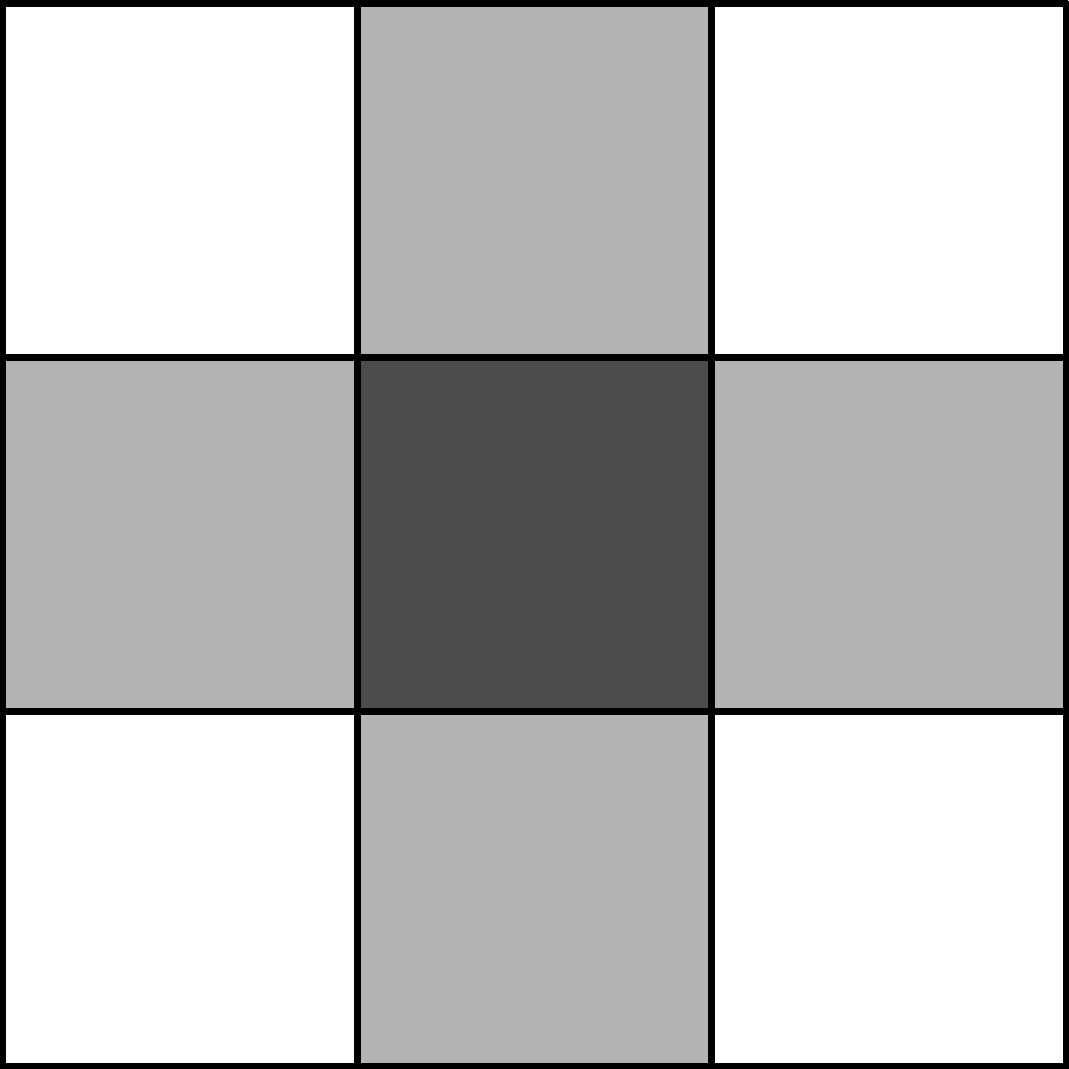
\includegraphics[width=0.5\columnwidth]{img/basics/connected-compontents/4-connectivity}
    \caption{4-Konnektivität}
  \end{subfigure}
  \begin{subfigure}{0.3\columnwidth}
    \centering
    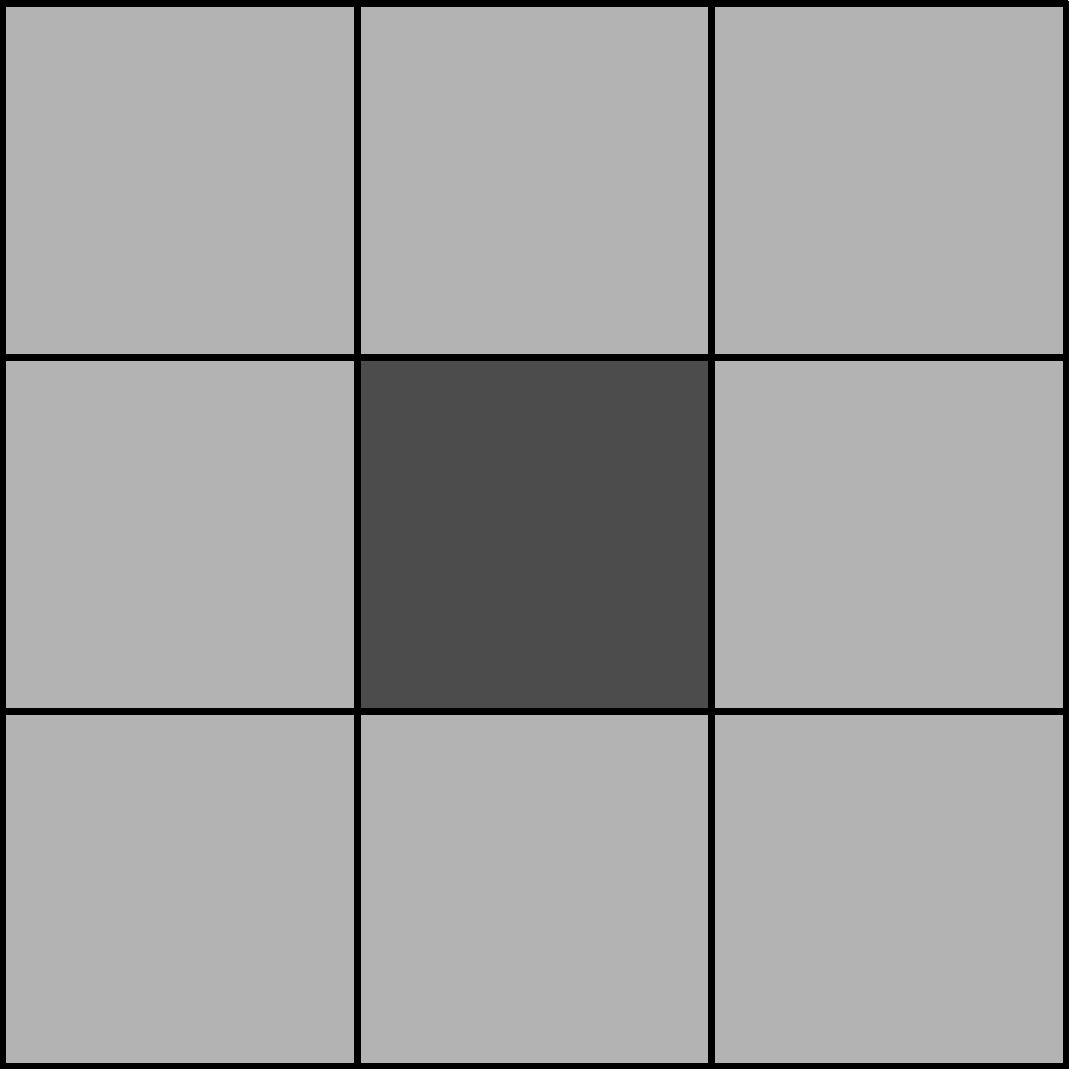
\includegraphics[width=0.5\columnwidth]{img/basics/connected-compontents/8-connectivity}
    \caption{8-Konnektivität}
  \end{subfigure}
  \caption[Vergleich von Pixelnachbarschaften]{Vergleich von Pixelnachbarschaften, mit dem betrachteten Pixel markiert in Dunkelgrau und den Pixeln der Nachbarschaft in Hellgrau.}
\end{figure}
%
Je mehr Pixel als Nachbarschaft herangezogen werden, desto größer können die zusammenhängenden Komponenten ausfallen, da es mehr Möglichkeiten gibt in denen zwei Pixel als verbunden gelten.

Das Connected-Component-Labeling ist realisierbar mittels eines Scanlineverfahrens~\cite[S.~69--75]{compvis2001}, d.h. jede Bildzeile wird, mit der oberen Zeile~($y=0$) beginnend, pixelweise von links~($x=0$) nach rechts verarbeitet.
Jedes Pixel wird auf Verbundenheit mit seinen Nachbarn~(4-Konnektivität) oberhalb~($y-1$) und links~($x-1$) geprüft.
Unterscheidet sich der Wert des aktuellen Pixels von den betrachteten Nachbarn so wird diesem ein neues Label zugewiesen.
Besitzt das Pixel hingegen den Wert mindestens eines Nachbarn so wird das Label des Nachbarn zugewiesen.
Besitzen mehrere Nachbarn den gleichen Wert aber unterschiedliche Label, so werden diese Label als äquivalent markiert.
Die erste Bildzeile und -spalte müssen gesondert initialisert werden, da diese keine Nachbarn oberhalb bzw. links besitzen.
Sind alle Pixel verarbeitet, müssen Labeläquivalenzen aufgelöst werden, sodass Pixeln mit äquivalenten Label ein gemeinsames Label zugewiesen werden kann. Zum Erfassen der Äquivalenzen eignet sich die UnionFind-Datenstruktur.
%
\begin{figure}[H]
  \centering
  \begin{subfigure}[t]{0.327\columnwidth}
    \centering
    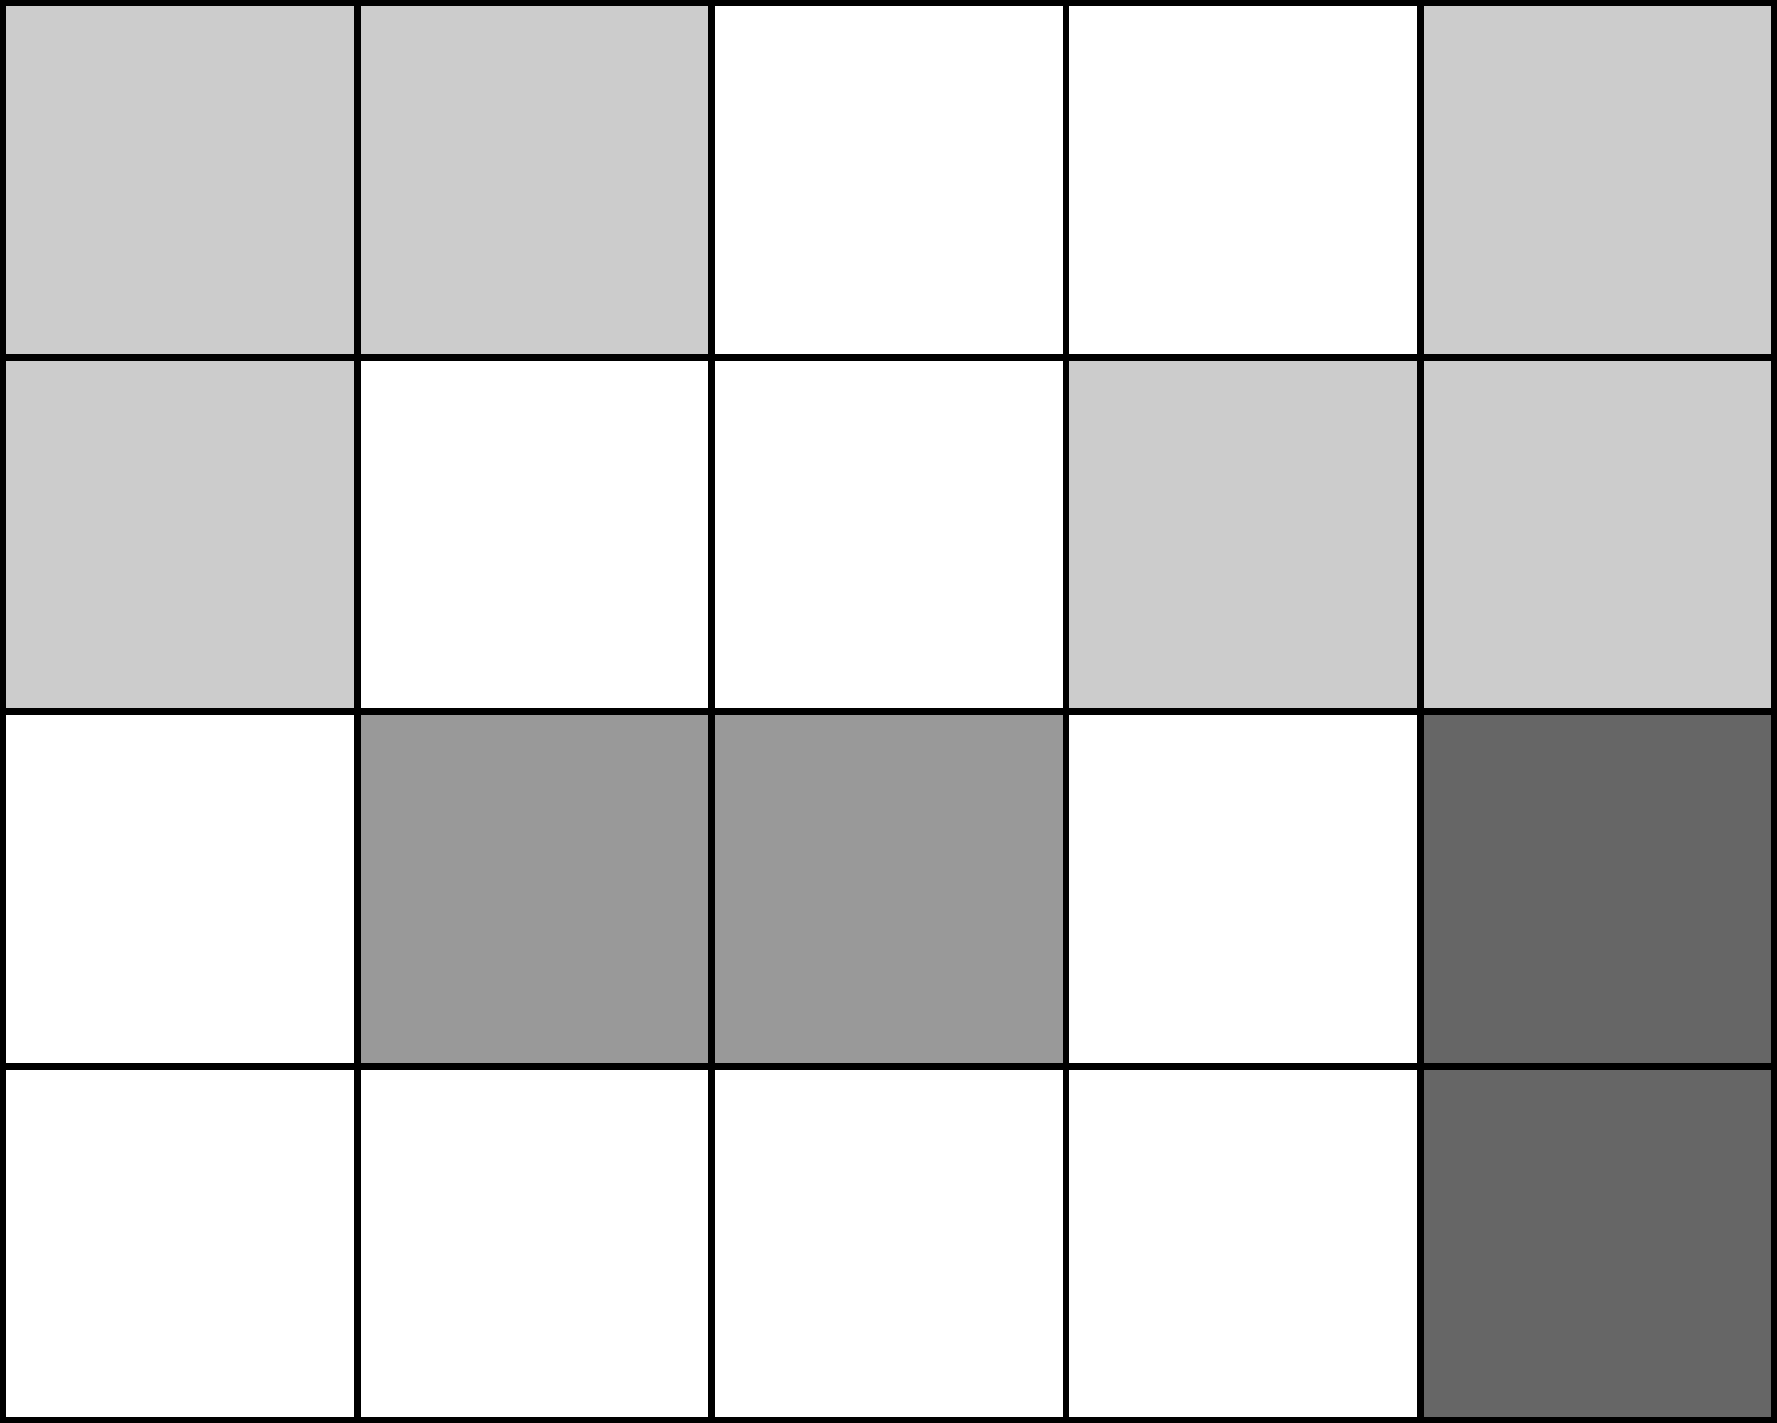
\includegraphics[width=\columnwidth]{img/basics/connected-compontents/labeling-1}
    \caption{Ausgangsgrafik}
  \end{subfigure}
  \begin{subfigure}[t]{0.327\columnwidth}
    \centering
    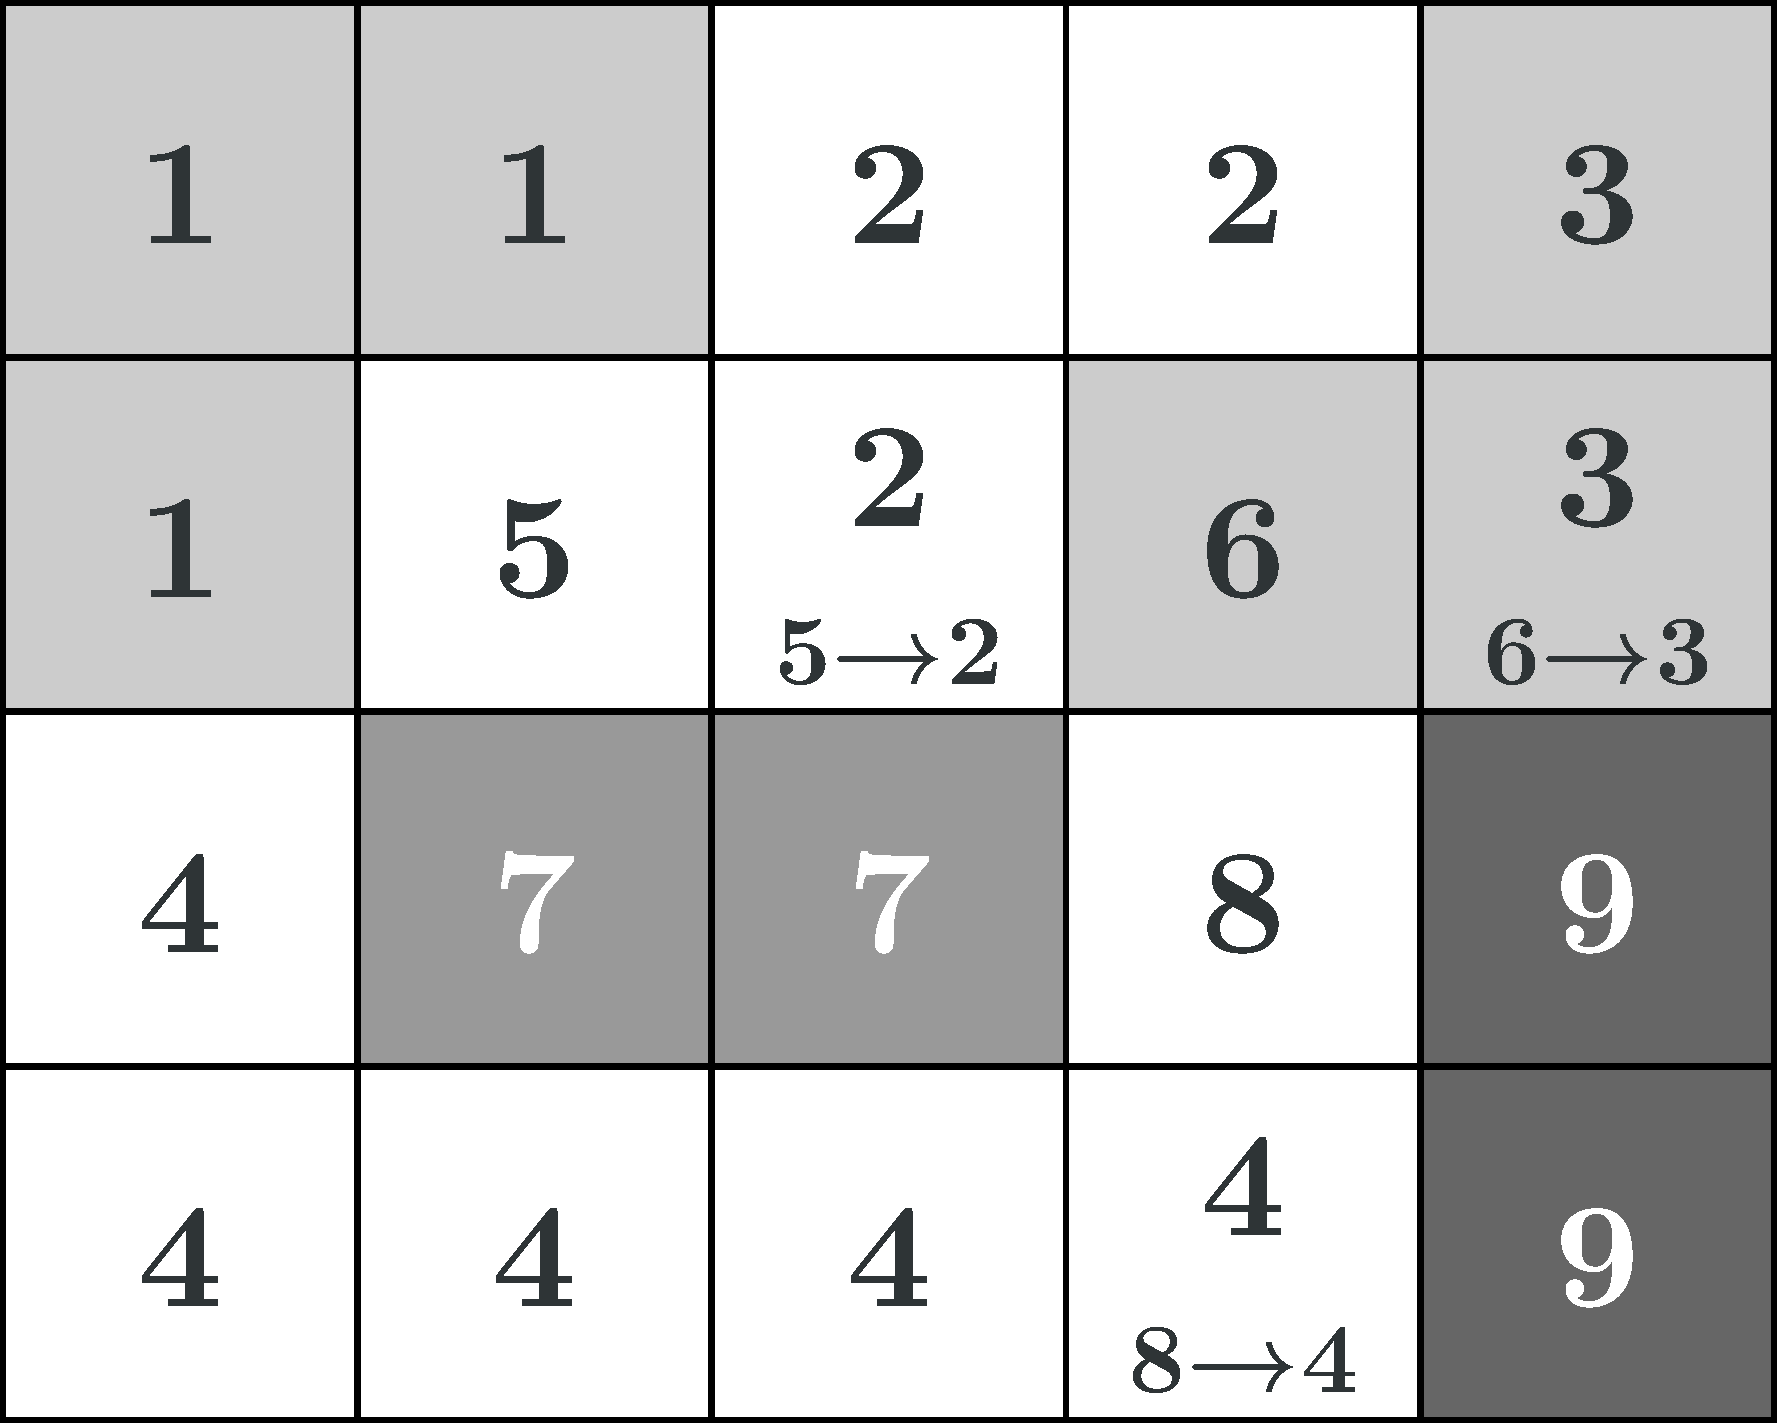
\includegraphics[width=\columnwidth]{img/basics/connected-compontents/labeling-2}
    \caption{Label zuweisen und Äquivalenzen ($\rightarrow$) aufzeichnen}
  \end{subfigure}
  \begin{subfigure}[t]{0.327\columnwidth}
    \centering
    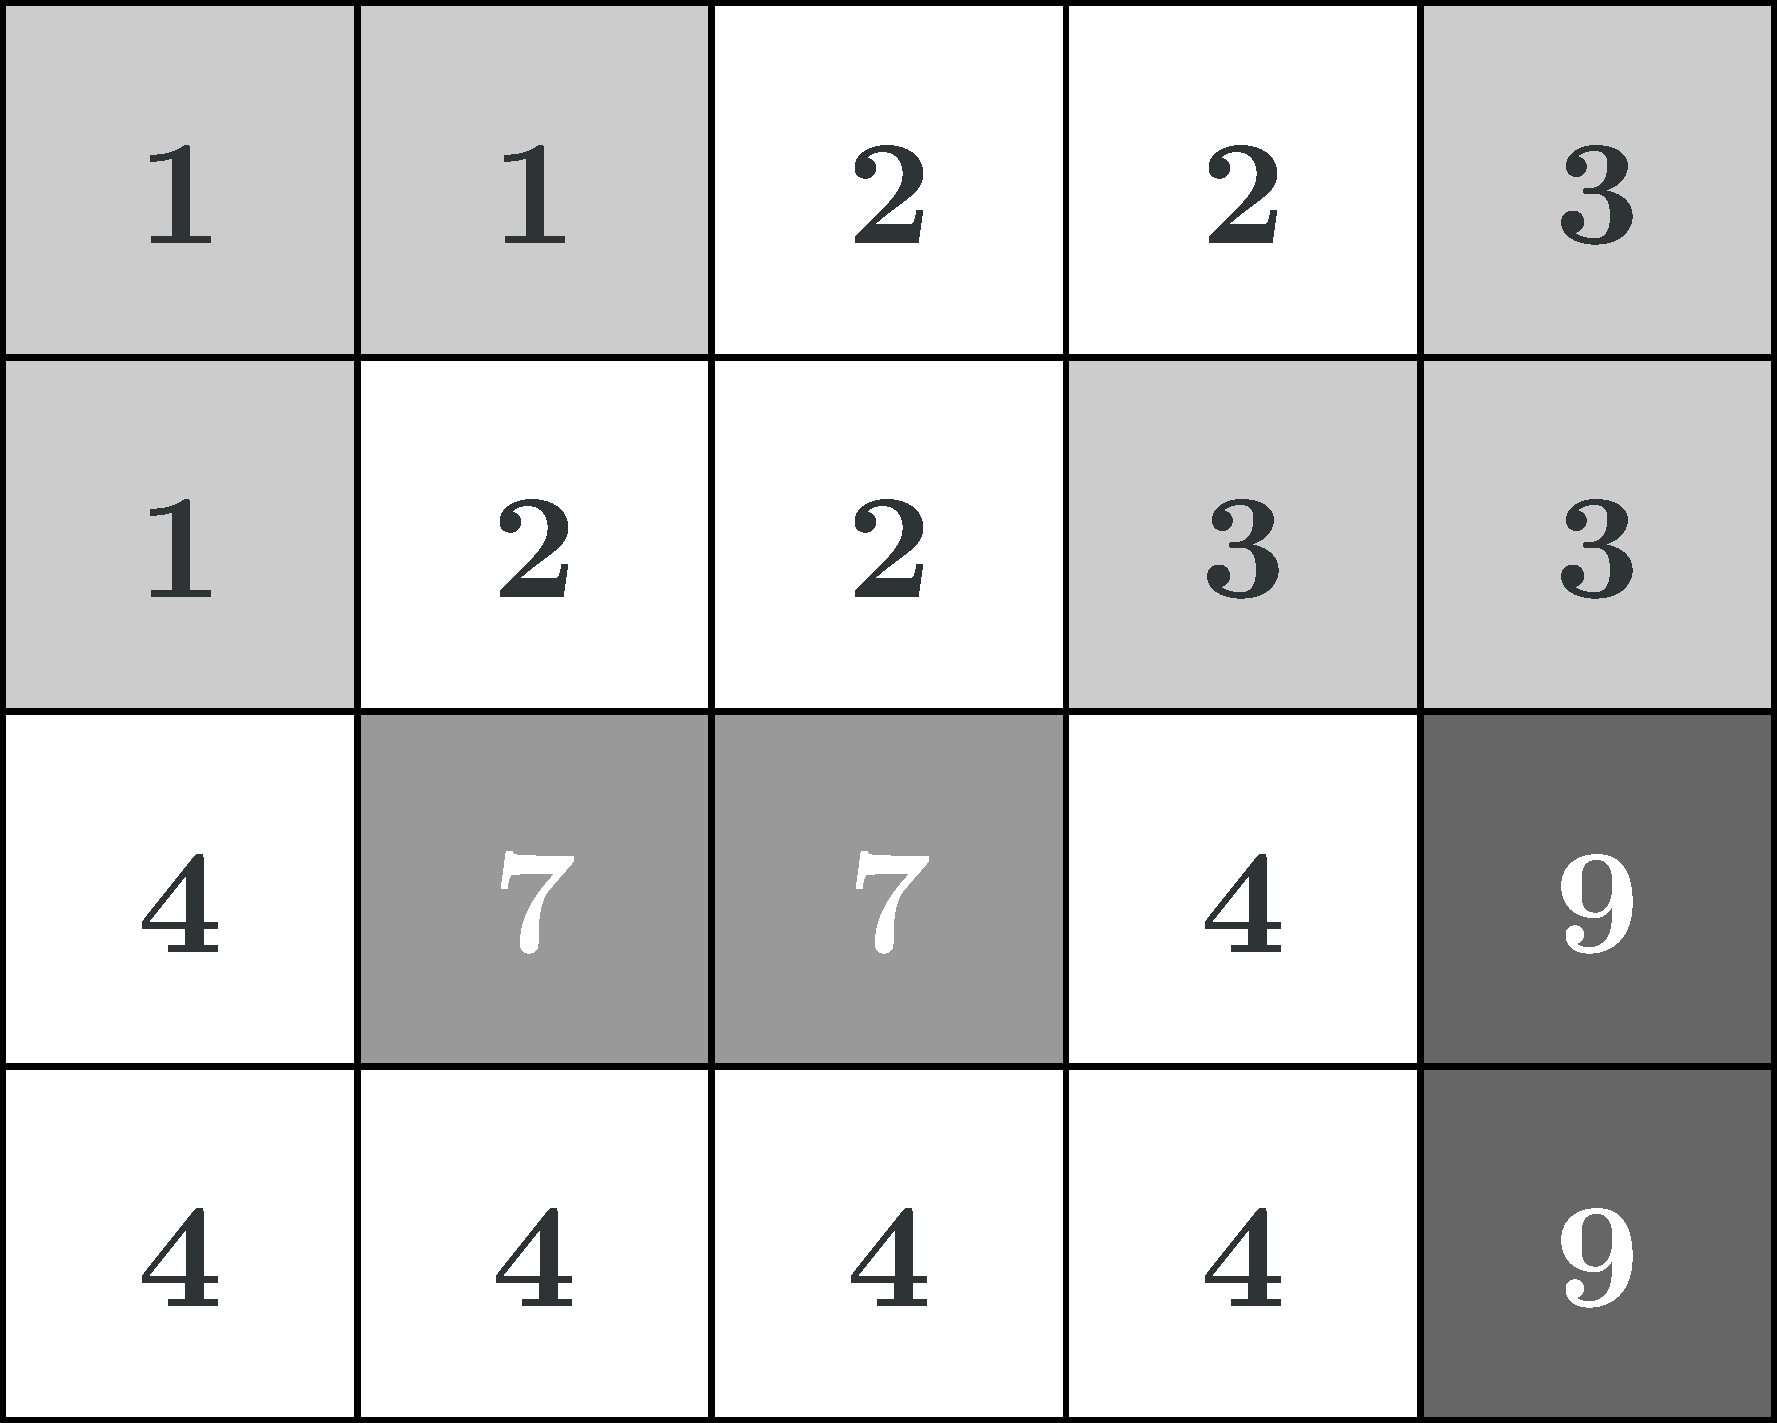
\includegraphics[width=\columnwidth]{img/basics/connected-compontents/labeling-3}
    \caption{Äquivalenzen auflösen}
  \end{subfigure}
  \caption[Ablauf des Connected-Components-Labeling]{Ablauf des Connected-Components-Labeling mit 4-Konnektivität.}
\end{figure}

\section{Konvexe Hülle}
\writtenby{\dcauthornameewie}%
Als konvexe Hülle einer Punktmenge $M$ bezeichnet man das minimale konvexe Polygon, welches sämtliche Punkte aus $M$ enthält.
Für die Berechnung der konvexen Hülle aus einer Menge von Punkten existieren diverse Alogirthmen.
Ein simpler Algorithmus ist \textsc{Andrew}'s Monotone Chain  \cite[6--7]{compgeom2008}.
Dazu werden zwei "`halbe"' Hüllen erstellt, die obere Hülle $U$ und untere Hülle $L$.
Die obere Hülle wird erzeugt indem über alle Punkte der Menge $M$ entsprechend ihrer lexikografischen Ordnung\footnote{
  \( (x,y) < (u, v) \Longleftrightarrow x < u \vee x = u \wedge y < v \)
} iteriert, und wiederholt das letzte Element in $U$ entfernt wird solange $U$ mindestens 2 Punkte enthält und die letzten 2 Punkte zusammen mit dem aktuell betrachteten Punkt \emph{keine} Rechtskurve bilden.
Anschließend wird der aktuelle Punkt ans Ende von $U$ eingefügt.
Die Erzeugung der unteren Hülle $L$ erfolgt analog $U$, jedoch unter Betrachtung der Punkte in umgekehrter Reihenfolge.
Zudem \emph{müssen} die letzten 2 Punkte zusammen mit dem aktuell betrachteten Punkt eine Rechtskurve bilden.
Abschließend werden $U$ und $L$ so zusammen gefasst, dass diese die konvexe Hülle als Liste von Eckpunkten im Uhrzeigersinn ergeben.

\section*{Filterprozesse}
\writtenby{\dcauthornameriren}%
Für viele Bildverarbeitungsprozesse werden Filter genutzt, die sich z.B. der mathematischen Faltung bedienen, um Rauschen zu entfernen, Kanten zu schärfen oder auch Kanten zu erkennen. Die wichtigsten der zur Verbesserung der Bildqualität genutzten Filter, werden hier kurz erläutert.

\todo{Übertragung und Vertiefung vom Implementierungsteil?}
\subsection*{Lineare Filter}

\subsection*{Faltungsfilter}

\subsection*{Gaußfilter}

\subsection*{Unscharfes Maskieren}

\subsection*{Laplacian of Gaussian}


